\section{Data Provenance Model}
\lstset{stringstyle=\color{black}}


\subsection{Existing Data Models}

\subsection{New Data Model}

We define a data point (DP) as a uniquely identifiable and addressable piece of data (i.e., a value) in the context of the smart grid. Examples for DPs in the context of smart grid includes sensor readings such as 3-phase electric currents, complex analytics results derived from sensor readings etc. The unique identifier is composed of three blocks.
\begin{itemize}
	\item Unique Identifier - A data point distinguishes itself specifically from other data flowing in the Data Provenance Model for smart grid  (e.g., bulk sensor readings that are of no further interest, ephemeral intermediary analytics results, etc.) in that it is addressable, i.e., it has an ID that is unique in the context of the smart grid. In order to ensure the uniqueness of the identifier, we came up with an identifier generation strategy, which generates a unique ten-byte identifier and ensures uniqueness across the system. Data point identifier comprised of:
		\begin{itemize}
			\item 3-byte node identifier - Guarantees its uniqueness across machines/nodes and processes.
			\item 4-byte value representing the seconds since the Unix epoch - Ensures uniqueness in relation to a single second.
			\item 3-byte counter - Provides uniqueness within a single second in a single process.
		\end{itemize}
		\subsection* {Properties} Our unique identifier mechanism along with its simplicity brought some other advantages and reduced the need to store machine/node identifier separately and also ease some time-based queries (e.g., sorting based on generation timestamp).
			\begin{itemize}				
				\item Example: 5a7b91370003c6badfb2
			\end{itemize}
	\item Input Data Points - A data point may be based on other data points that have contributed to its creation or modification. We refer to these related
data points as input data points(IDP). A data point's IDP is a list of unique identifiers of all those data points, which contributed to its creation or transformation. It also stores information about the contribution type.
	
	\begin{itemize}			
			\item Example: 
\begin{lstlisting}			
[{
    "average": [   // Contribution type
        "5a81c07800031ddaf123",
        "5a81c09300031d341fab"
    ]
}]		
\end{lstlisting}
	\end{itemize}
	\item Context - Specific context for provenance may vary for different IoT applications. We propose a data model for the context in typical IoT environments comprising the concepts of Agents, Execution Context, as well as Time and Location information. An Agent is an entity that creates and/or modifies data points (e.g., sensor, software agent, device, etc.). It is recursively defined in such a way that an agent can contain other agents (e.g., a device containing several sensors). This recursion allows for defining agents in a hierarchy and may be used as fine-grained as required. For instance, an agent hierarchy may span from the concept of a particular function in a software library running over a virtualization container on a particular device to a particular IoT network.
		
\begin{figure}[h]
\centering
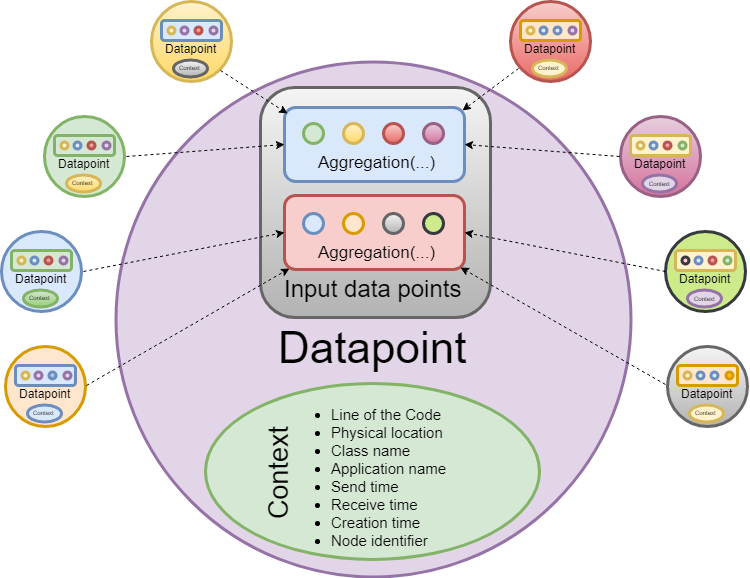
\includegraphics[width=\linewidth]{figures/dataModelforIDP.png}\\
\caption{Data Model}
\label{dataModel}
\end{figure}
\end{itemize}
TODO